\documentclass[12pt, twoside]{article}
\usepackage[francais]{babel}
\usepackage[T1]{fontenc}
\usepackage[latin1]{inputenc}
\usepackage[left=7mm, right=7mm, top=7mm, bottom=7mm]{geometry}
\usepackage{float}
\usepackage{graphicx}
\usepackage{array}
\usepackage{multirow}
\usepackage{amsmath,amssymb,mathrsfs}
\usepackage{soul}
\usepackage{textcomp}
\usepackage{eurosym}
 \usepackage{variations}
\usepackage{tabvar}

\begin{document}


\section*{\center{Aide individualis�e: Pourcentages}}

\subsection*{Coefficient multiplicateur}

Soit $a=10$.

\begin{enumerate}
  \item Multiplier $a$ par 1,04.
  
  Compl�ter: 1,04 \ldots 1
  
  Le nombre obtenu est plus \ldots \ldots \ldots que $a$.
  \item Multiplier $a$ par 0,8.
  
  Compl�ter: 0,8 \ldots 1
  
  Le nombre obtenu est plus \ldots \ldots \ldots que $a$.  
  \item Multiplier $a$ par 0,61.
  
  Compl�ter: 0,61 \ldots 1
  
  Le nombre obtenu est plus \ldots \ldots \ldots que $a$.  
  \item Multiplier $a$ par 1,97.
  
  Compl�ter: 1,97 \ldots 1
  
  Le nombre obtenu est plus \ldots \ldots \ldots que $a$. 
\end{enumerate}

\medskip

Compl�ter les phrases:

\enskip

\fbox{
\begin{minipage}{18cm}
\begin{itemize}
  \item [$\bullet$] Lorsque je multiplie un nombre positif $a$ par un nombre
  plus grand que \ldots, le r�sultat obtenu est un nombre \ldots \ldots \ldots
  \ldots \ldots \ldots que le nombre $a$.
  \item [$\bullet$] Lorsque je multiplie un nombre positif $a$ par un nombre
  plus petit que \ldots, le r�sultat obtenu est un nombre \ldots \ldots \ldots
  \ldots \ldots \ldots que le nombre $a$.  
\end{itemize}
\end{minipage}
}

\subsection*{Calculer un pourcentage}

Calculer 8 \% de 300 c'est trouver $x$ dans le tableau de proportionnalit�
suivant: \begin{tabular}{|c|c|}
\hline
8 & 100 \\
\hline
$x$ & 300 \\
\hline
\end{tabular}

\enskip

On trouve alors $x=\ldots \ldots$. 

On peut aussi directement appliquer la formule ce qui est plus rapide: 8 \% de
300$= \dfrac{8}{100} \times 300$

\enskip

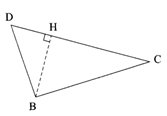
\includegraphics[width=9cm]{images/ex4.jpg}

\subsection*{Applications}

\subsubsection*{Exercice 1}

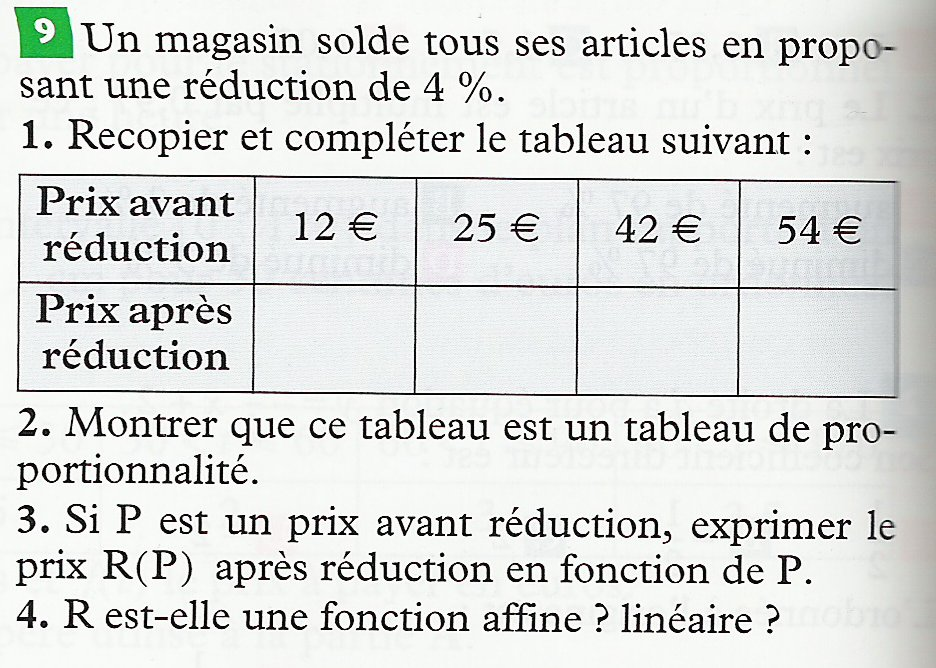
\includegraphics[width=9cm]{images/ex9.jpg}

\subsubsection*{Exercice 2}


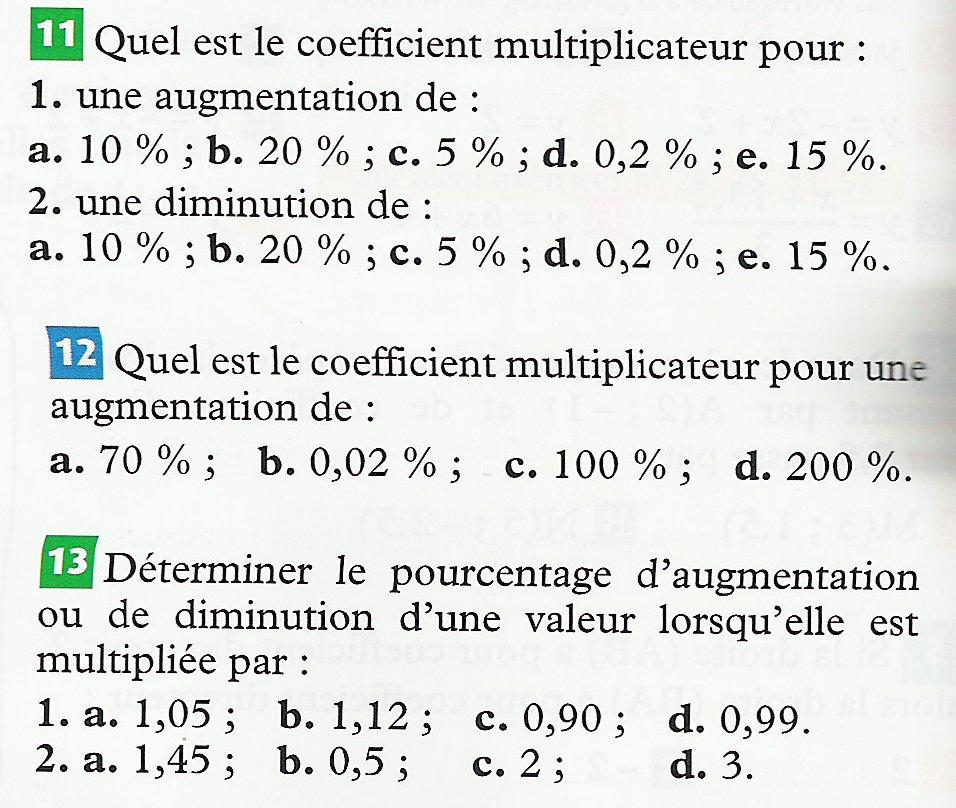
\includegraphics[width=9cm]{images/ex11.jpg}

\subsubsection*{Exercice 3}

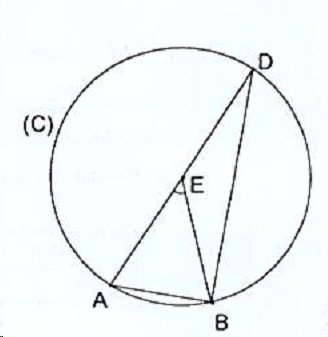
\includegraphics[width=9cm]{images/ex3.jpg}


\end{document}
